\documentclass[../views.tex]{subfiles}

\begin{document}

Een logical view is een omschrijving van de functionaliteiten die de eindgebruiker gebruikt \parencite{architectural_blueprints}. De diagrammen omschrijven dus niet altijd een volledige programma. De logical views van de frontend, collector en server zijn respectievelijk te vinden in \autoref{fig:logical_view_frontend}, \autoref{fig:logical_view_collector} en \autoref{fig:logical_view_server}.

Er zijn twee legenda's: een voor de frontend, en een voor de collector en server. Dit is gedaan omdat de programmeertaal Go klassen noch objecten kent, maar Typescript wel.

% Frontend
\begin{figure}[ht]
  \centering
  \fbox{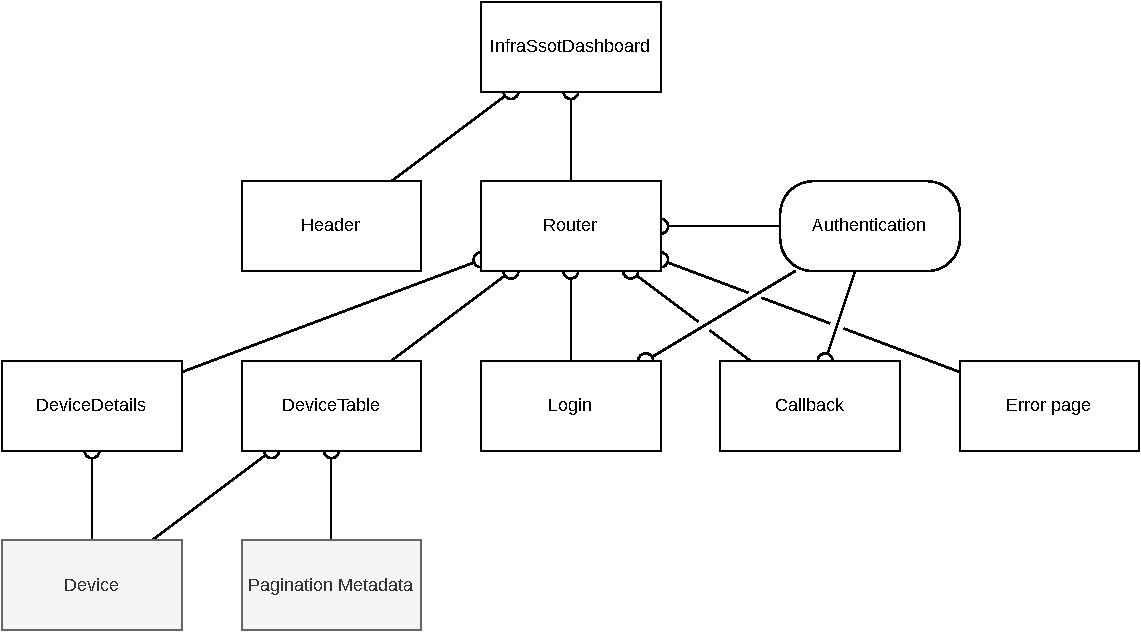
\includegraphics[width=0.95\textwidth]{assets/images/drawio/logical view frontend.pdf}}
  \caption{De logical view van de frontend.}
  \label{fig:logical_view_frontend}
\end{figure}

% Preact legenda
\begin{figure}[ht]
  \centering
  \fbox{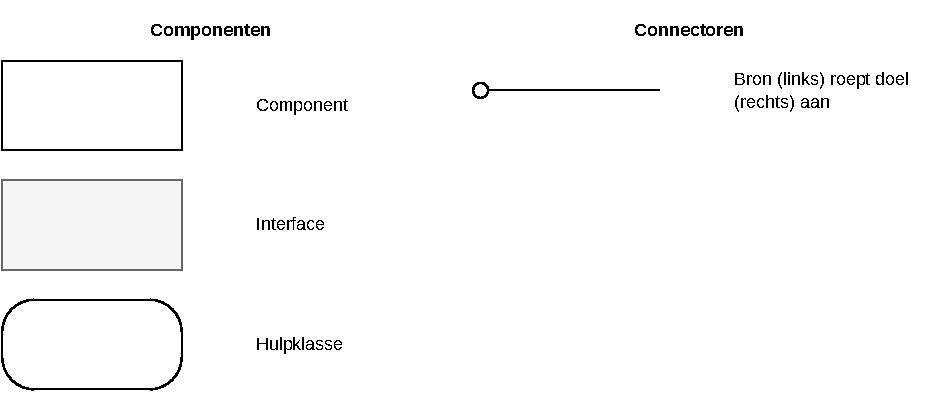
\includegraphics[width=0.95\textwidth]{../assets/images/drawio/logical view legend preact.pdf}}
  \caption{Legenda voor \autoref{fig:logical_view_frontend}.}
\end{figure}

% Collector
\begin{figure}[ht]
  \centering
  \fbox{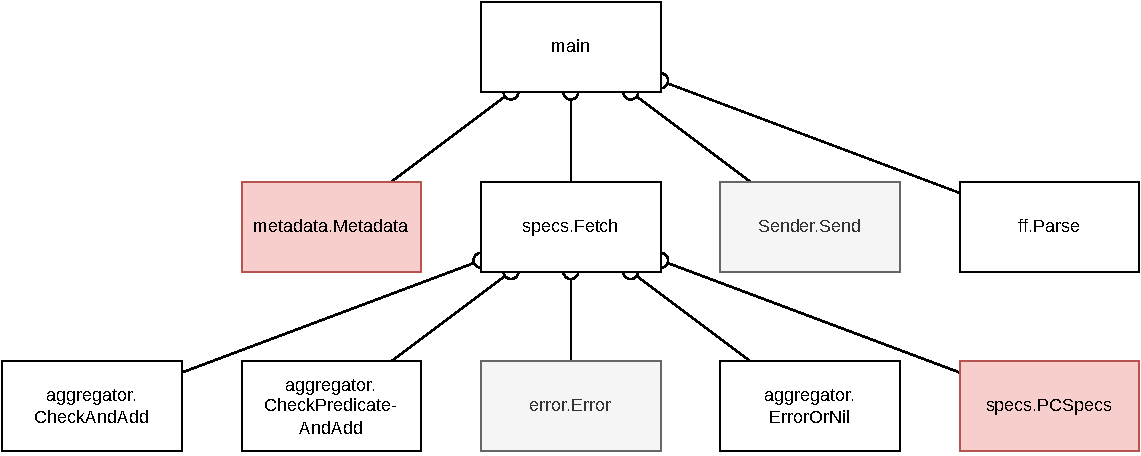
\includegraphics[width=0.95\textwidth]{../assets/images/drawio/logical view collector.pdf}}
  \caption{De logical view van de collector.}
  \label{fig:logical_view_collector}
\end{figure}

% Server
\begin{figure}[ht]
  \centering
  \fbox{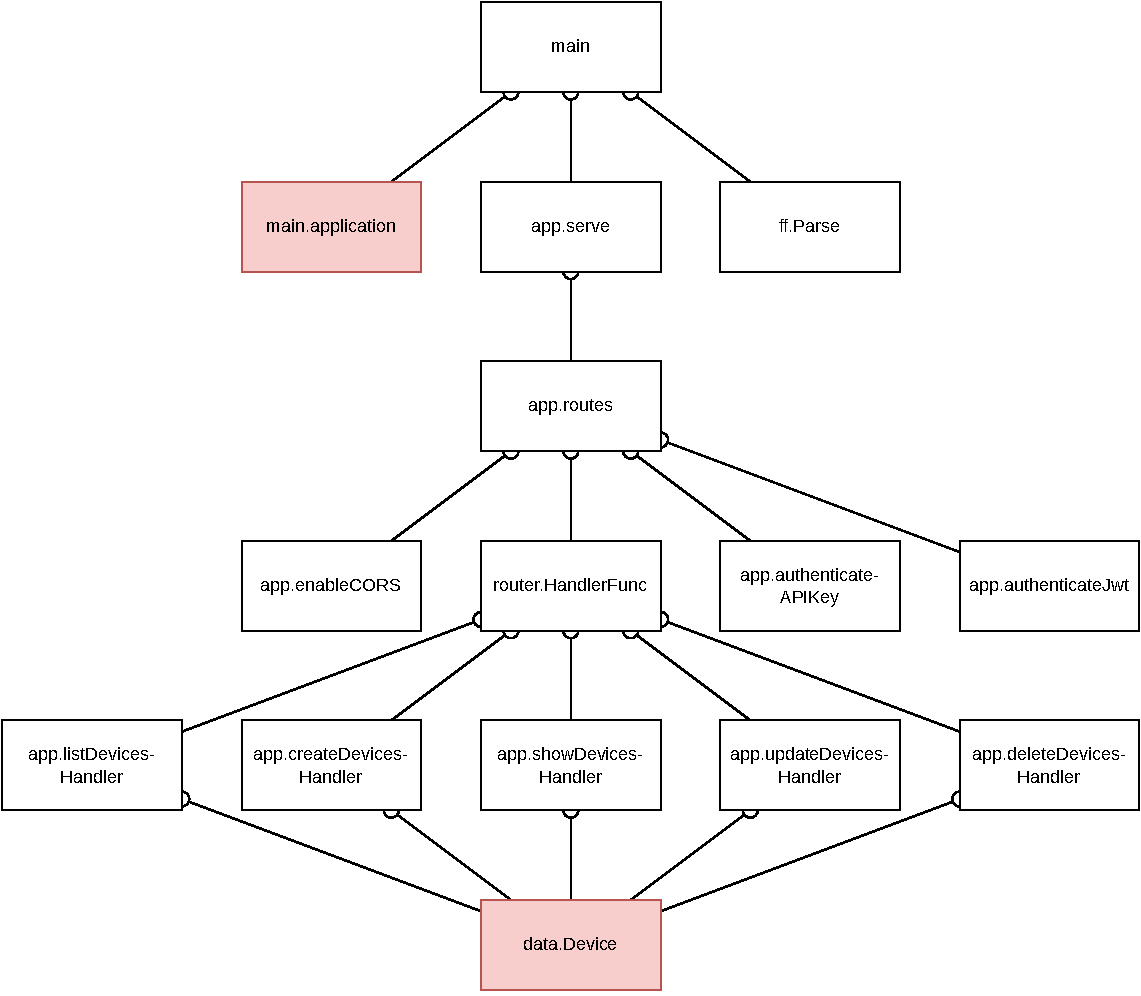
\includegraphics[width=0.95\textwidth]{../assets/images/drawio/logical view server.pdf}}
  \caption{De logical view van de server.}
  \label{fig:logical_view_server}
\end{figure}

% Go legenda
\begin{figure}[ht]
  \centering
  \fbox{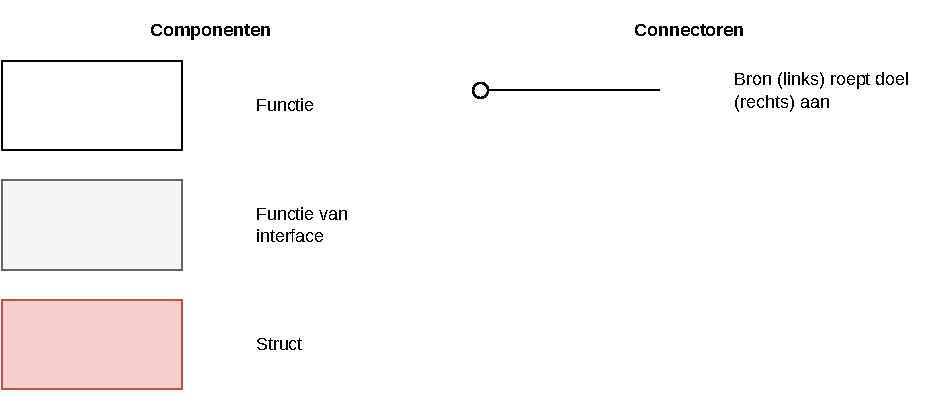
\includegraphics[width=0.95\textwidth]{../assets/images/drawio/logical view legend go.pdf}}
  \caption{Legenda voor \autoref{fig:logical_view_collector} en \ref{fig:logical_view_server}.}
\end{figure}

\end{document}
